% !TeX spellcheck = en_GB
% encoding: utf8
% !TEX encoding = utf8
% !TEX program = pdflatex
% !BIB program = biber

\documentclass[11pt,oneside,a4paper]{report}

\usepackage[utf8]{inputenc}
\usepackage[T1]{fontenc}
\usepackage[colorlinks]{hyperref}
\usepackage[left=2.5cm, right=2.5cm, top=2.5cm, bottom=2.5cm]{geometry}
\usepackage{float}
\usepackage{subcaption}
\usepackage{mathtools}
\usepackage{color}
\usepackage[backend=biber,maxnames=10,style=numeric,sorting=nty,abbreviate=false,giveninits=true,language=english]{biblatex}

\addbibresource{../meros.bib}

%\newcommand{\twc}[1]{\textcolor{red}{\textbf{TW}: #1}}
\newcommand{\Fig}[1]{Fig.~\ref{#1}}

\definecolor{amber}{rgb}{1.0, 0.49, 0.0}
\newcommand{\twci}[1]{
	\textcolor{amber}{TW: #1}}

% encoding: utf8
%
% Stereotypes
%

% Lista powinna być zgodna z profilem w EA

\newcommand{\stActionConn}{<<Action>>}
\newcommand{\stCommChannel}{<<CommChannel>>}
\newcommand{\stComponContain}{<<ComponContain>>}
\newcommand{\stGpPackages}{<<GpPackages>>}
\newcommand{\stHardware}{<<Hardware>>}
\newcommand{\stLaunchFile}{<<LaunchFile>>}
\newcommand{\stMetaPackage}{<<MetaPackage>>}
\newcommand{\stMicroNode}{<<MicroNode>>}
\newcommand{\stNamespace}{<<Namespace>>}
\newcommand{\stNode}{<<Node>>}
\newcommand{\stPackage}{<<Package>>}
\newcommand{\stParameter}{<<Parameter>>}
\newcommand{\stRepository}{<<Repository>>}
\newcommand{\stRosCommCompon}{<<RosCommCompon>>}
\newcommand{\stRosConn}{<<RosConn>>}
\newcommand{\stRQtNode}{<<RQtNode>>}
\newcommand{\stRunSystemCompon}{<<RunSystemCompon>>}
\newcommand{\stServiceConn}{<<Service>>}
\newcommand{\stSourExeContain}{<<SourExeContain>>}
\newcommand{\stSystem}{<<System>>}
\newcommand{\stTerminal}{<<Terminal>>}
\newcommand{\stTopicConn}{<<Topic>>}
\newcommand{\stWorkspace}{<<Workspace>>}

\newcommand{\stblock}{<<block>>}





\begin{document}
	
\title{MeROS: SysML-based Metamodel for ROS-related Systems - version 4.0.0 - reference manual}
\author{MeROS developers group - https://github.com/twiniars/MeROS \\ tomasz.winiarski@pw.edu.pl}
\date{\today}
\maketitle


\begin{abstract}
	The complexity of today's robot control systems implies difficulty in developing them efficiently and reliably. Systems engineering (SE) and frameworks come to help. The frameworks' metamodels are needed to support the standardisation and correctness of the created application models. MeROS is a~metamodel for ROS, which addresses the running system and developer workspace. An essential addition to the original ROS concepts is the grouping of these concepts, which provides an opportunity to illustrate the system's decomposition and varying degrees of detail in its presentation. The metamodel is derived from the requirements and verified on the practical examples. The matter is described in a~standardised way in SysML (Systems Modeling Language). Hence, common development tools that support SysML can help develop robot controllers in the spirit of SE.
\end{abstract}
	
	
	
	\maketitle
	
\chapter*{Important citation notice}

\textbf{If you are to use MeROS in your papers, please first cite the IEEE ACCESS  article~\cite{meros-access}, where the initial version of the MeROS is presented. You can also refer to MeROS project page \cite{meros-www} and mention the actual MeROS version you are using.}
	
	
\chapter{Introduction}
\label{ch:intro}	

	The development of civilisation has led to an increase in the importance of robotics. Many modern robotic systems are complex. To create them as effectively and reliably as possible, it is necessary to follow systems engineering (SE), where metamodels play an essential role~\cite{bezivin2004search,kent2002model,schmidt2006model}.
	Robots, especially complex ones, are mostly controlled with usage of software. Hence, in robotics, SE is inextricably linked with software engineering, where frameworks have been crucial for many years \cite{mnkandla2009software,shehory2014agent}.
	Diverse robotics frameworks have been developed so far \cite{hentout2016survey,inigo2012robotics,tsardoulias2017robotic}. Some steps towards standardisation have been made in recent years, and ROS (Robot Operating System) has come to the fore, currently in ROS~2 version \cite{maruyama2016exploring,park2020real}.   
	
	The robotic models can be subdivided~\cite{de2021survey} into Platform Independent Models (PIM), e.g., \cite{tasker2020,earl2020,zielinski2010motion,zielinski2017variable}, and Platform Specific Models (PSM). The metamodels of ROS, including MeROS, belong to PSM and should answer to the component nature of ROS \cite{Figat:2022:RAS,wenger2016model}.
	 MeROS is founded on SysML (Systems Modeling Language) \cite{Friedenthal:2015,omg-sysml17}, a~profile of UML (Unified Modeling Language). Modelling in languages from the UML family addresses a~number of important aspects of systems engineering \cite{chaudron2012effective}. These include the use cases [UCX]:
	\begin{itemize}
		\item $[$UC1] Systems' documentation and presentation,
		\item $[$UC2] Effective analysis of systems, especially in interdisciplinary teams (graphical language is more understandable for non-specialists in the field), 
		\item $[$UC3] Defects detection,
		\item $[$UC4] Integration of new collaborators into the development team,
		\item $[$UC5] Resuming work after a~break,
		\item $[$UC6] Extension and modification of existing systems,
		\item $[$UC7] Support the implementation of new systems,
		\item $[$UC8] Migration of systems.
	\end{itemize}
	
	In practice, documentation is created both prior to implementation and, in many cases, through a~process of reverse  engineering \cite{canfora2007new} for existing systems. Agile-type strategies involve modifying the documentation as the project develops \cite{habib2021systematic}. Systems development with V-model-based application of MeROS metamodel was proposed in \cite{winiarski2025-v-model}.
			
	The following presentation was prepared basing on the diagrams created as the core of the Visual Paradigm project. It starts with formulating the requirements (chapter~\ref{ch:requirements}). These requirements are allocated to the MeROS metamodel that's architecture is described in chapter~\ref{ch:architecture}. The applications of MeROS are presented in other documents.
	MeROS metamodel can be employed in various ways in broad context of SE. To help to develop projects, the MeROS Visual Paradigm stereotypes and other materials are accessible from MeROS project page\footnote{\url{http://github.com/twiniars/meros}}. 
	
	
\chapter{MeROS requirements}
\label{ch:requirements}
	The requirements [RX] formulation process for MeROS metamodel is multi-stage and iterative. In the beginning, the initial requirements were formulated based on: (i) literature review (both scientific and ROS wiki/community sources), (ii) author experience from supervising and supporting ROS-related projects, and finally, (iii) author experience from EARL (Embodied Agent-based cybeR-physical control systems modelling Language) \cite{earl2020} PIM development and its applications (e.g. \cite{tasker2020,karwowski2021hubero,en14206693-grav-comp}). Verification of subsequent versions of MeROS by its practical applications led to an iterative reformulation of the following requirements and respective MeROS architecture.
	
	MeROS requirements are depicted on a~number of dedicated SysML diagrams. The requirements are organised in a~tree-like nesting structure, with additional internal relations, and labelled following this structure. The general requirements are presented in Fig.~\ref{fig:general_req}. 
		
	\begin{figure}[H]
		\centering
		\begin{center}
			{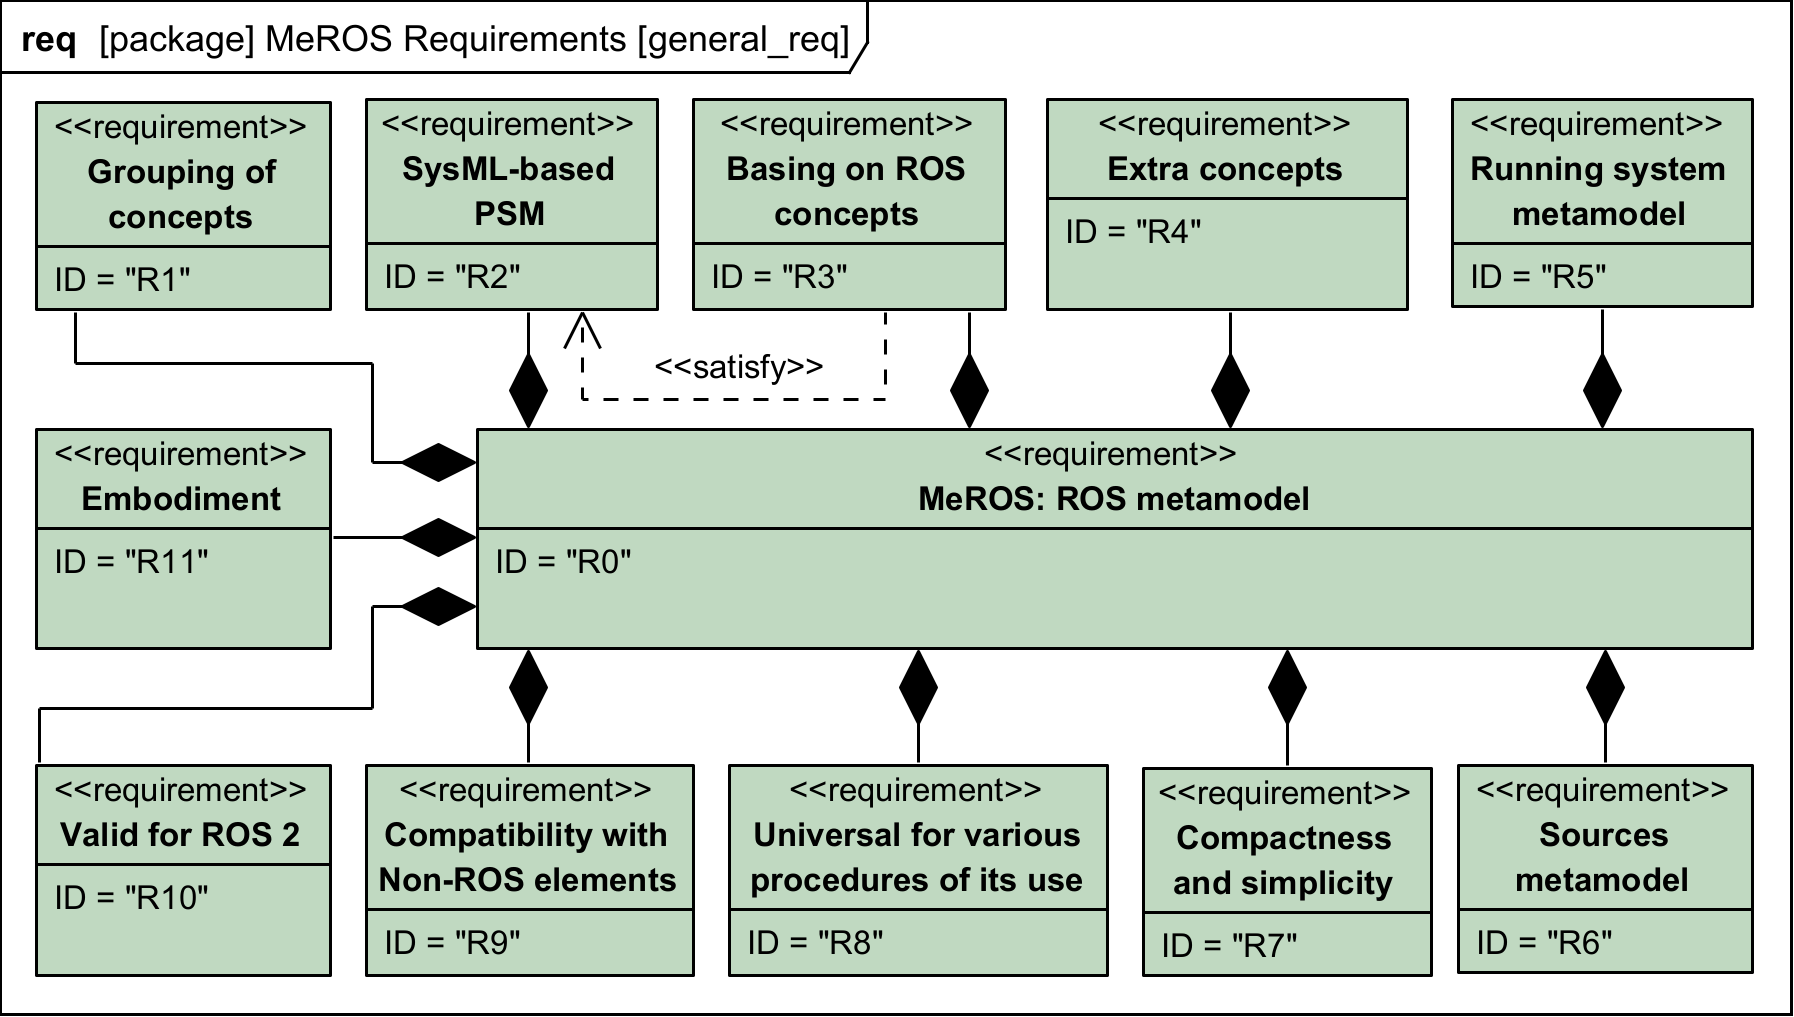
\includegraphics[scale=1.0]{diagrams/general_req.png}}
		\end{center}
		\caption{General requirements.}
		\label{fig:general_req}
	\end{figure}
		
	Grouping of concepts [R1] is a crucial addition to pure ROS metamodel. 
	MeROS is a  SysML-based metamodel and is classified into PSM [R2].
	 MeROS aims to cover ROS concepts [R3] and not change their labels as long as possible, to maintain conformity and intuitiveness. To achieve completeness of the metamodel extra concepts are needed [R4]. The ROS system is two-faced. While it is executed [R5], it has a~specific structure and behaviour, but from the developers' point of view, the sources [R6] are the exposed aspect. The model should be compact and straightforward [R7] rather than unnecessarily elaborate and complicated. It is also universal. It does not imply itself the specific procedure of its use [R8]. These procedures are specified outside of the MeROS metamodel. Although the SysML-based MeROS is classified into PSM, it should be compatible with Non-ROS elements [R9]. MeROS metamodel should be valid for ROS~2 [R10]. Finally, embodiment [R11] (e.g. system deployment) should be considered.
	
	The grouping of concepts requirements are presented in Fig.~\ref{fig:grouping_req}. It has diverse aims. It enables the presentation of the system part in a~general, PIM-like abstract way, on the logical level rather than a~detailed, PSM-like implementation one. The aggregation reduces the number of objects represented on the diagram to highlight the essential aspects and stay compact and consistent in presentation.
	
	\begin{figure}[H]
		\centering
		\begin{center}
			{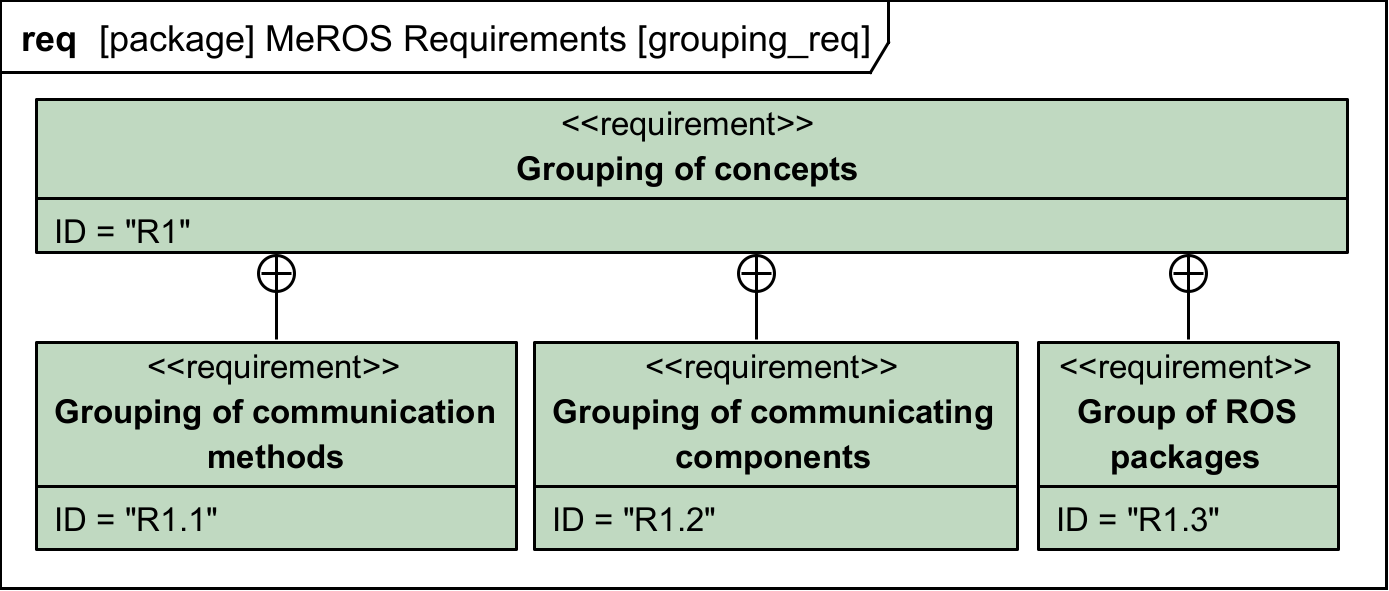
\includegraphics[scale=1.0]{diagrams/grouping_req.png}}
		\end{center}
		\caption{Grouping of concepts requirements.} 
		\label{fig:grouping_req}
	\end{figure}
	
	A~vital addition to the original ROS concepts is the abstract grouping of:  (i) communication methods and (ii) communicating components and ROS packages.  It should be noted that several ROS concepts group other concepts in a~particular way, especially to deploy the system. Action aggregates Topics and Services, Component Container aggregates Nodes.

		
	The ROS concepts that MeROS models are organised into four major classes (Fig.~\ref{fig:ros_concepts_req}): (i)~Communicating components, (ii) Communication methods, (iii) Sources containers, and (iv) Other.
	

	\begin{figure}[H]
		\centering
		\begin{center}
			{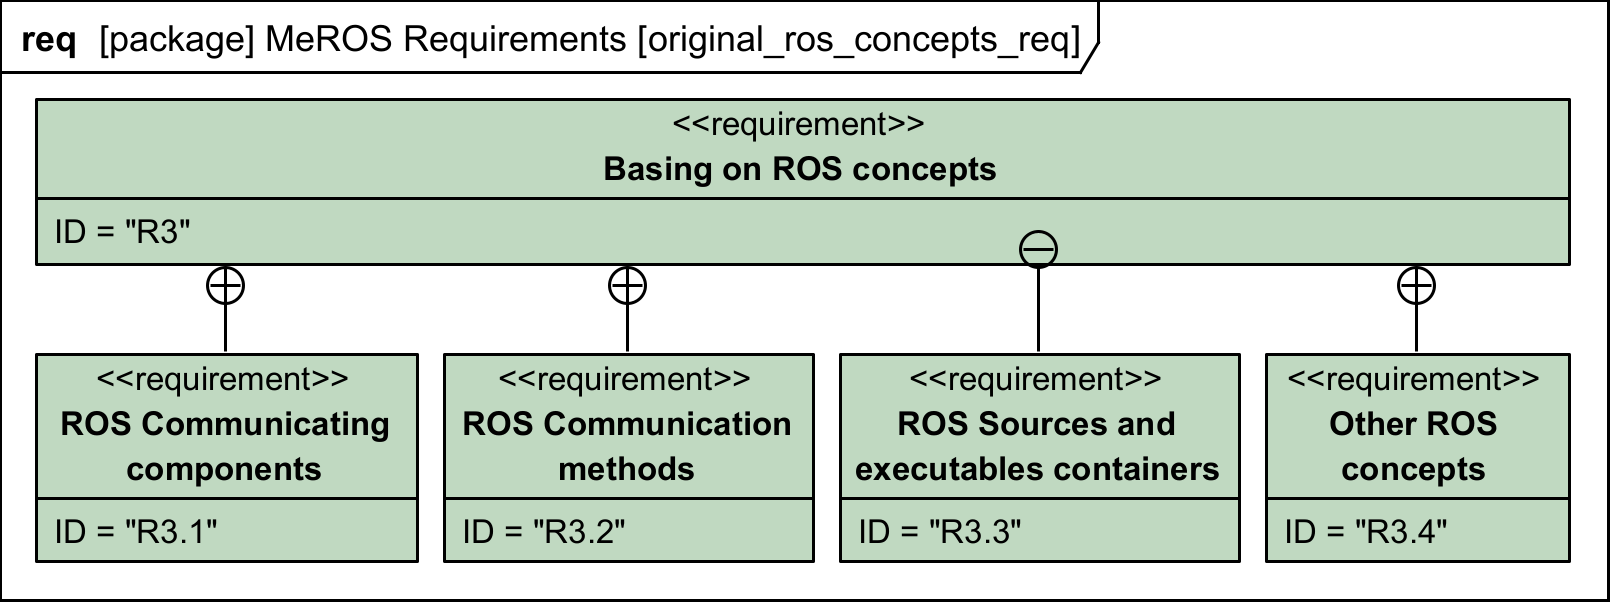
\includegraphics[scale=1.0]{diagrams/original_ros_concepts_req.png}}
		\end{center}
		\caption{ROS concepts requirements.} 
		\label{fig:ros_concepts_req}
	\end{figure}

	\pagebreak
	
	 ROS Node is member of ROS Communicating components [R3.1]  (Fig.~\ref{fig:communicating_components_req}).

	\begin{figure}[H]
		\centering
		\begin{center}
			{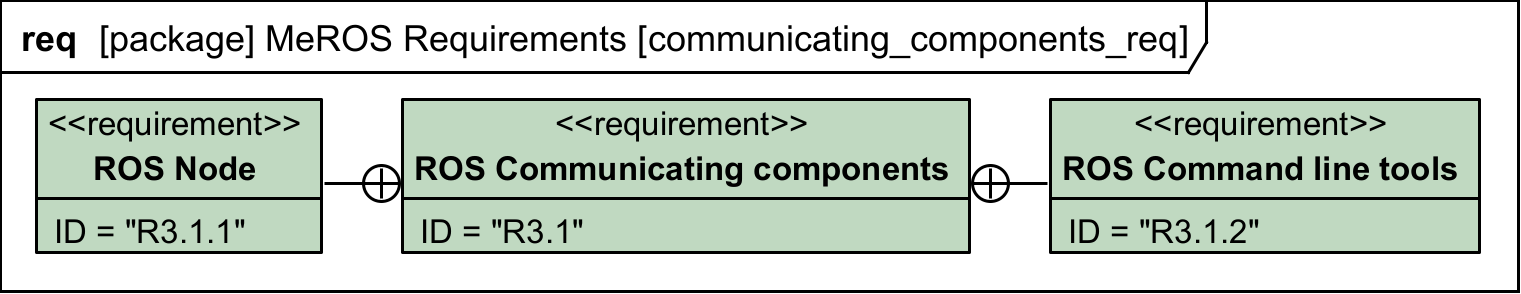
\includegraphics[scale=1.0]{diagrams/communicating_components_req.png}}
		\end{center}
		\caption{Communicating components requirements.} 
		\label{fig:communicating_components_req}
	\end{figure}
	
	Communication methods are depicted in Fig.~\ref{fig:communication_concepts_req}.
	 Three methods of communication are considered with their inter-component connections and data structures: (i) ROS Topic, its Message and connection, (ii) ROS Service comprising data structure and connection, and finally (iii) ROS Action including data structure and connection.
	
	\begin{figure}[H]
		\centering
		\begin{center}
			{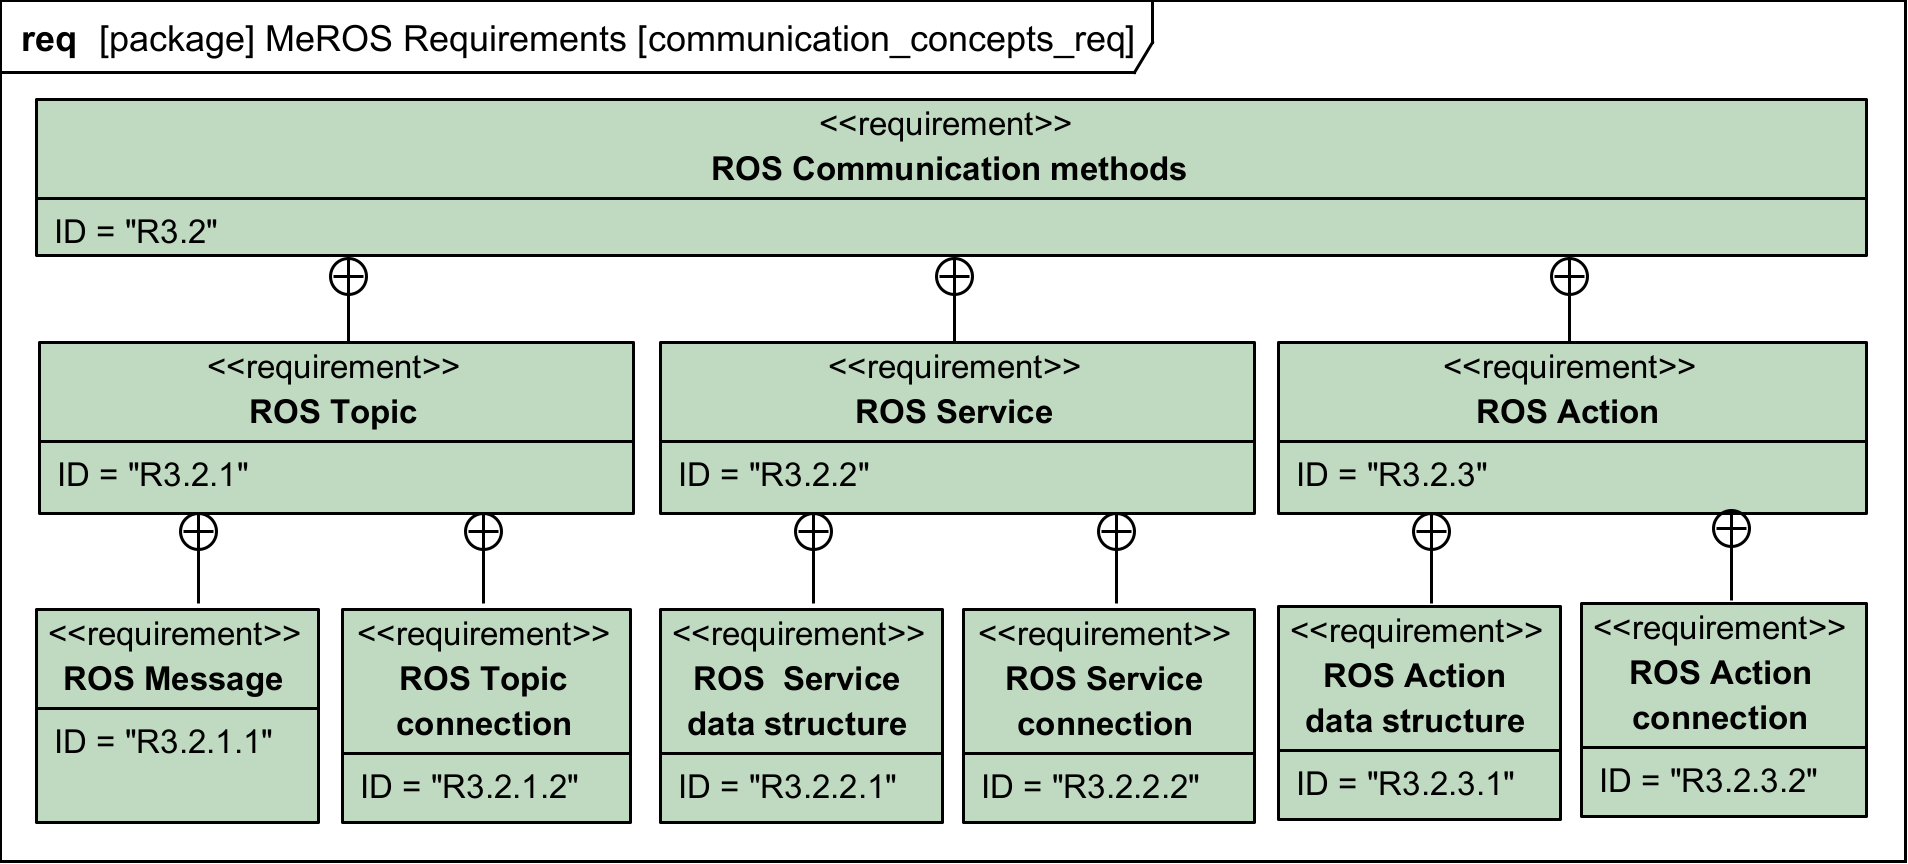
\includegraphics[scale=.98]{diagrams/communication_concepts_req.png}}
		\end{center}
		\caption{Communication concepts requirements.} 
		\label{fig:communication_concepts_req}
	\end{figure}
	
	ROS Sources containers comprises (Fig.~\ref{fig:sources_containers_req}): (i) ROS Package, (ii) ROS Metapackage, (iii) Group of ROS packages. It also relates to Group of packages and Repository. In practise ROS Metapackage is a~specific, degenerated ROS Package.
	
	\begin{figure}[H]
		\centering
		\begin{center}
			{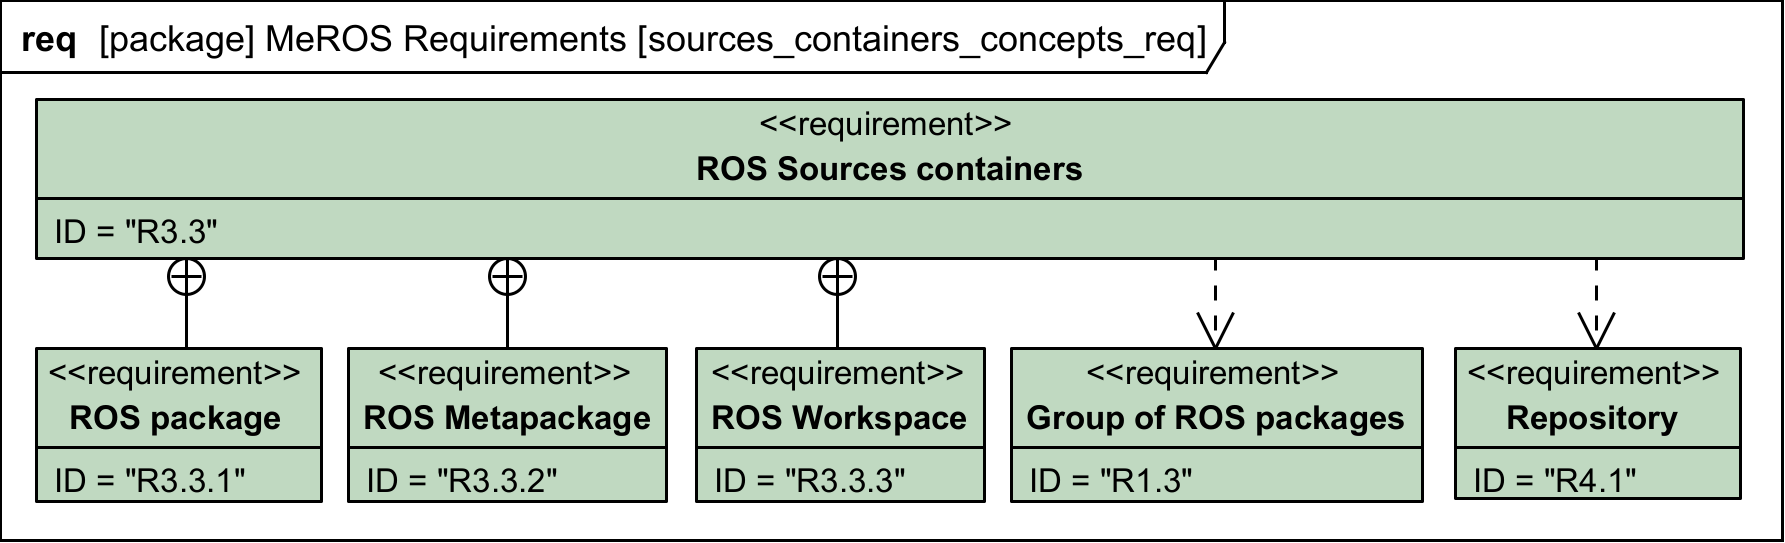
\includegraphics[scale=1.0]{diagrams/sources_containers_concepts_req.png}}
		\end{center}
		\caption{ROS Sources containers requirements.} 
		\label{fig:sources_containers_req}
	\end{figure}
	
	\pagebreak
	
	Other ROS concepts (Fig.~\ref{fig:other_ros_concepts_req}) include two elements: (i) ROS Parameters, (ii) ROS Namespace reflects the ROS concept to organise nodes and communication connections.
	
	\begin{figure}[H]
			\centering
			\begin{center}
					{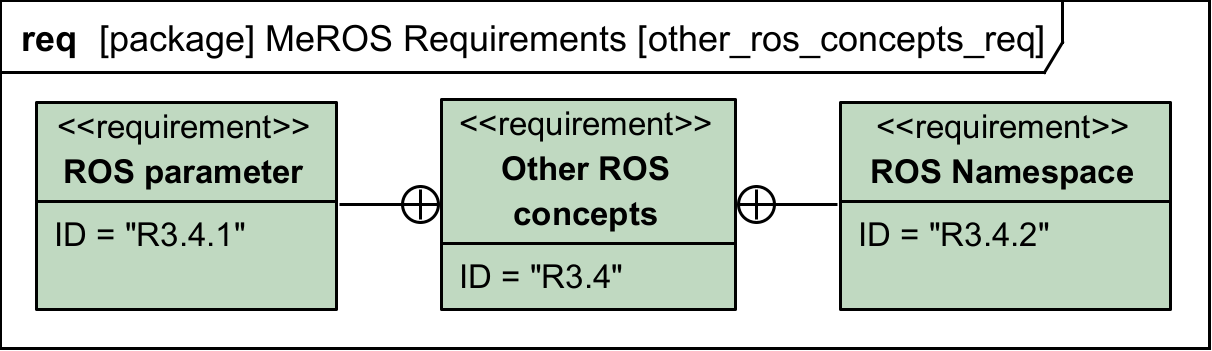
\includegraphics[scale=1.0]{diagrams/other_ros_concepts_req.png}}
				\end{center}
			\caption{Other ROS concepts requirements.} 
			\label{fig:other_ros_concepts_req}
		\end{figure}

Extra concepts are depicted in Fig.~\ref{fig:extra_concepts_req}.

\begin{figure}[H]
	\centering
	\begin{center}
		{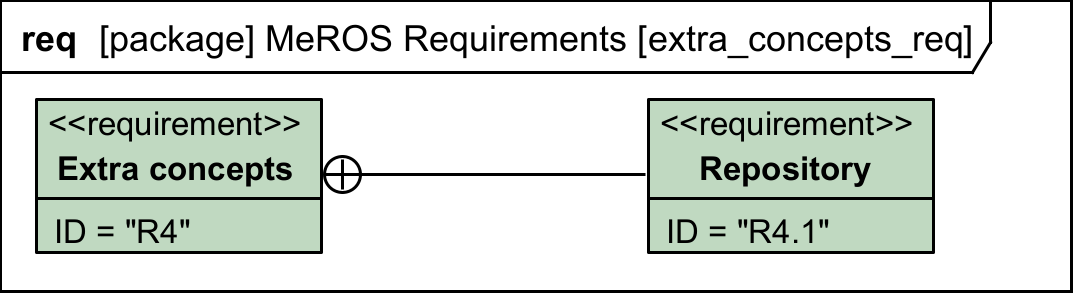
\includegraphics[scale=1.0]{diagrams/extra_concepts_req.png}}
	\end{center}
	\caption{Extra concepts requirements.} 
	\label{fig:extra_concepts_req}
\end{figure}


	To achieve intuitiveness, MeROS presents a~Running system structure (Fig.~\ref{fig:running_system_req}) following ROS rqt\_graph pattern. In particular, there are two ways to visualise communication, including and without	dedicated communication components.
	\begin{figure}[H]
		\centering
		\begin{center}
			{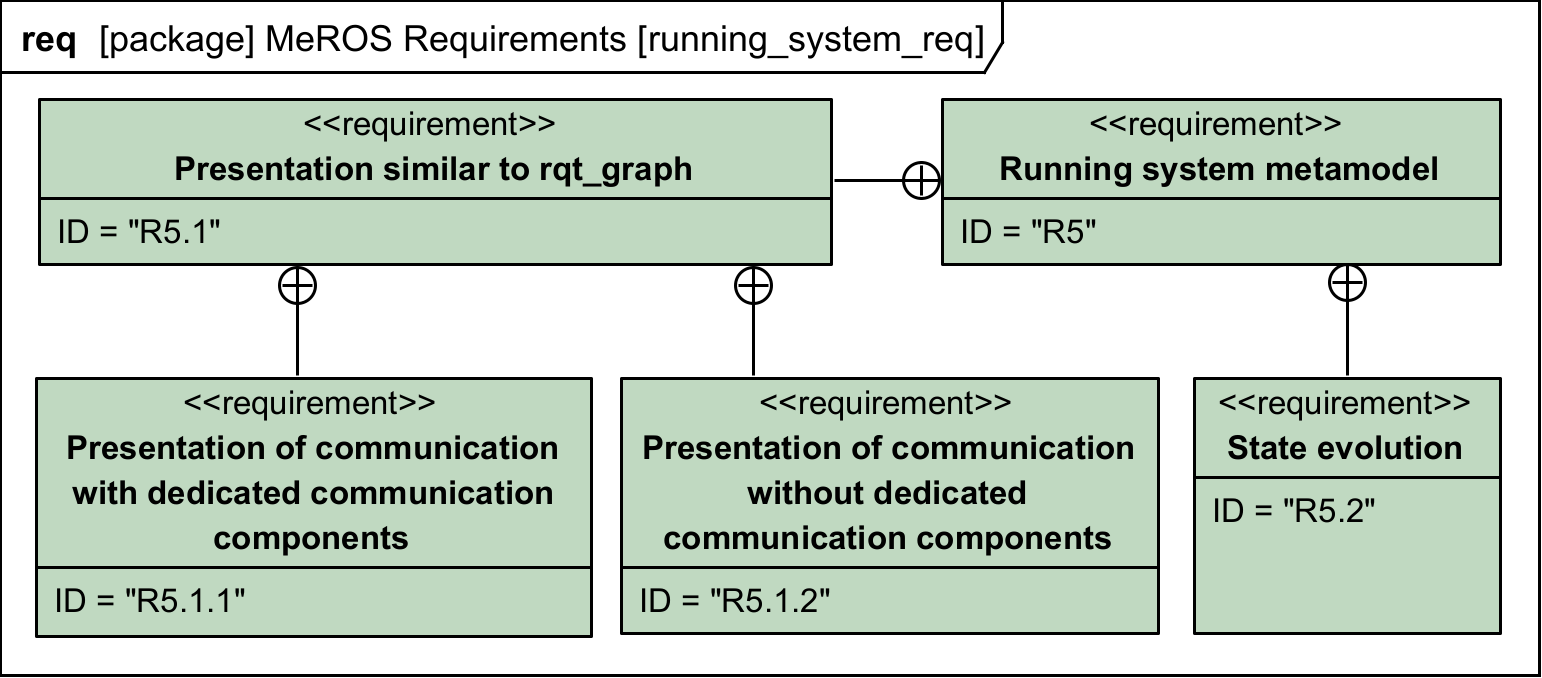
\includegraphics[scale=1.0]{diagrams/running_system_req.png}}
		\end{center}
		\caption{Running system requirements. } 
		\label{fig:running_system_req}
	\end{figure}
	 The dedicated components are especially useful in the presentation when many communication components use the same topic both on the publisher and the subscriber side. In opposition, the expression of topic names on arrows connecting communicating components, i.e., without dedicated communication components, let to reduce the number of components needed to depict communication for many topics and a~low number of communicating components. The other advantage of using dedicated communication components is that the particular connection can be split into several diagrams (e.g. ibd (internal block diagram) or sd (sequence diagram)), where the same object represents this connection in every associated diagram. Services and actions should be depicted as an addition to the presentation of the particular topics. It should be noted that rqt\_graph represents actions as a~number of topics and services. In MeROS, the topics and services being part of an action can be aggregated, which reduces the number of depicted connections.
		
	The compactness and simplicity and its nesting requirements are presented in Fig.~\ref{fig:compactness_and_simplicity_req}. 
	
	\begin{figure}[H]
		\centering
		\begin{center}
			{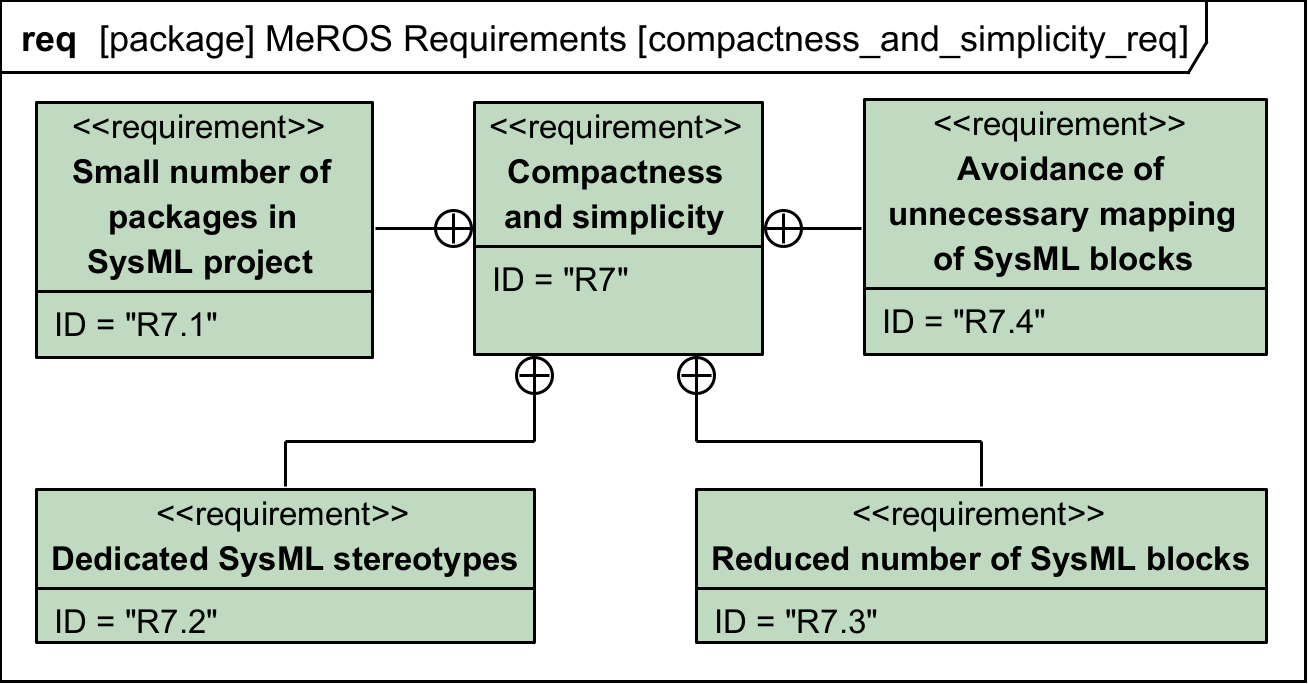
\includegraphics[scale=1.0]{diagrams/compactness_and_simplicity_req.png}}
		\end{center}
		\caption{Compactness and simplicity requirements.} 
		\label{fig:compactness_and_simplicity_req}
	\end{figure}
	
	A SysML project to develop and represent MeROS metamodel should consist of a~small number of packages, but still the packages should distinguish the major aspects of development process: (i) metamodel requirements formulation, (ii) metamodel itself, and (iii) metamodel realisations/applications.
	Dedicated SysML stereotypes [R6.2] are introduced to MeROS to replace the direct block specialization representation on diagrams and improve the legibility and compactness of diagrams.
	The number of SysML blocks should be reduced to a~reasonable level. Both [R7.1] and [R7.3] help in the Avoidance of unnecessary mapping of SysML blocks.

	
	
\chapter{MeROS architecture}
\label{ch:architecture}

	MeROS architecture is formulated according to the requirements discussed in the previous section. The diagrams comprise selected requirements being allocated to expose the MeROS metamodel development process. 
	The MeROS diagrams were created in the Visual Paradigm development tool within the SysML project [R8] and organised in two packages [R7.1]: (i) MeROS Requirements related to requirements formulation and analysis, (ii) MeROS Architecture.
		
	The stereotypes are introduced in MeROS metamodel [R7.2].
	The stereotypes names are created to compromise the descriptiveness and short length. Hence, the ROS phrase is avoided in stereotypes as long as there is only the ROS concept of a~given type.
	
	The degree of specificity of a~metamodel is a~compromise between its comprehensiveness (and, therefore, more general formulation) and a~more accurate representation of a~particular subclass of specific implementations. The metamodel contains compositions of elements and other primary relationships. Attributes and operations of elements range widely, hence their inclusion would lead to overgrowth and complication of the metamodel [R7]. The MeROS Metamodel is lightweight and general for various system development procedures and non-ROS parts of the whole System. The fundamental decision was to make it compact, so due to the extremely wide range of Non-ROS context variants [R9], they are specific for particular applications and are not specified in the metamodel itself. Hence, models derived from the metamodel can define their stereotypes, operations and new relations specific to a~particular System. 
	
	The SysML blocks reflects concepts pointed out in requirements, and their composition is depicted in block definition diagrams (bdd). Sources Containers (specialised especially by Workspaces) and Running System Components are composed into System (Fig.~\ref{fig:ros_system_bdd}). Hardware block reflects to embodiment. System can aggregate other Systems.
	
		
	\begin{figure}[H]
		\centering
		\begin{center}
			{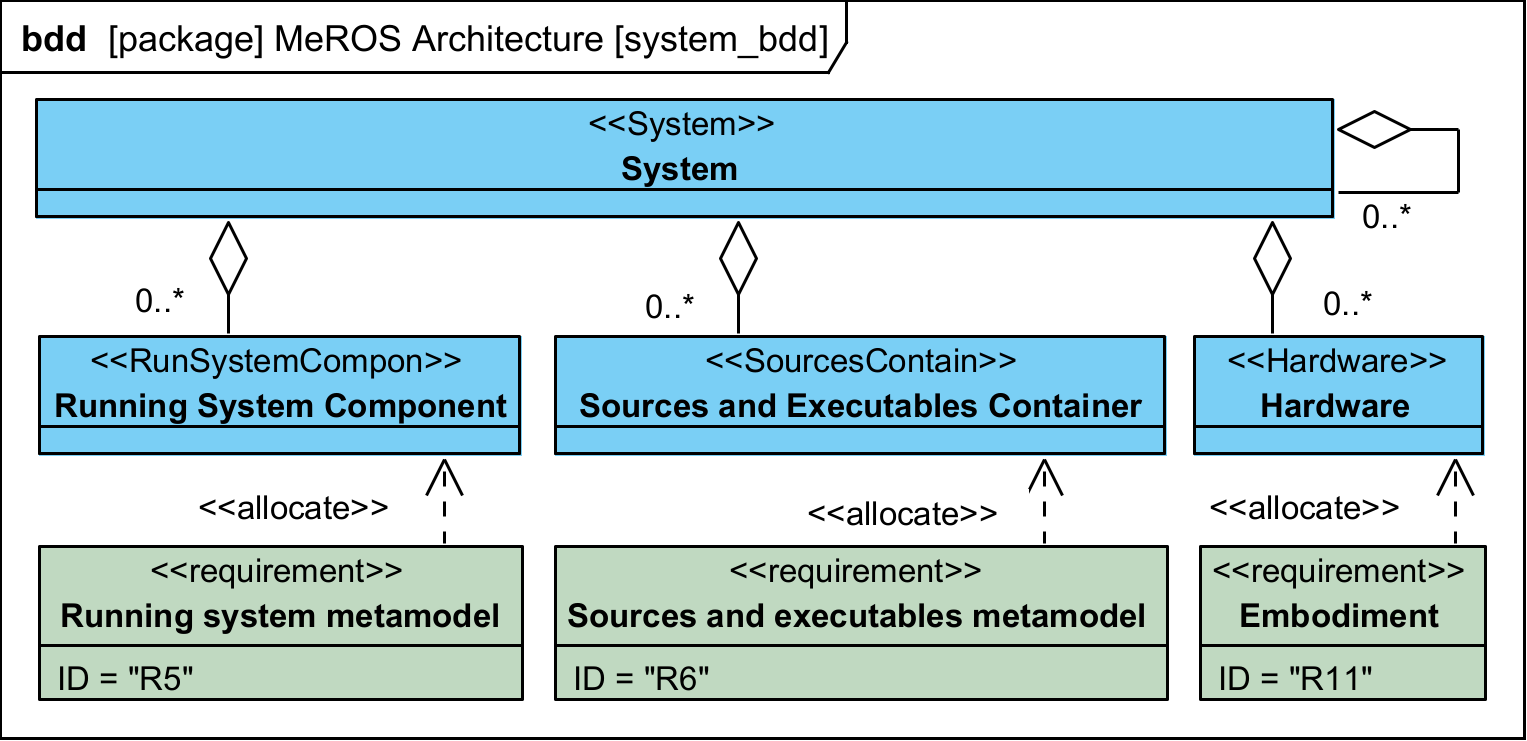
\includegraphics[scale=.98]{diagrams/system_bdd.png}}
		\end{center}
		\caption{System general composition.} 
		\label{fig:ros_system_bdd}
	\end{figure}
	
	Consequently, some concepts (e.g., Node), a~specialisations of Running System Component, occur in Sources Containers. It reduces the number of SysML blocks in the metamodel [R7.3] and eliminates the need for unnecessary mapping of SysML blocks [7.4]. In MeROS applications, the System formulation methodology is to create various views on it (in particular its: sources containers, running components, embodiment). They all together depict the complete view on the System.
	
	In MeROS, ROS Communicating Component (Fig.~\ref{fig:communicating_components_bdd}) forms a~crucial generalisation to represent standardised role regarding communication. 
	
		
	\begin{figure}[H]
		\centering
		\begin{center}
			{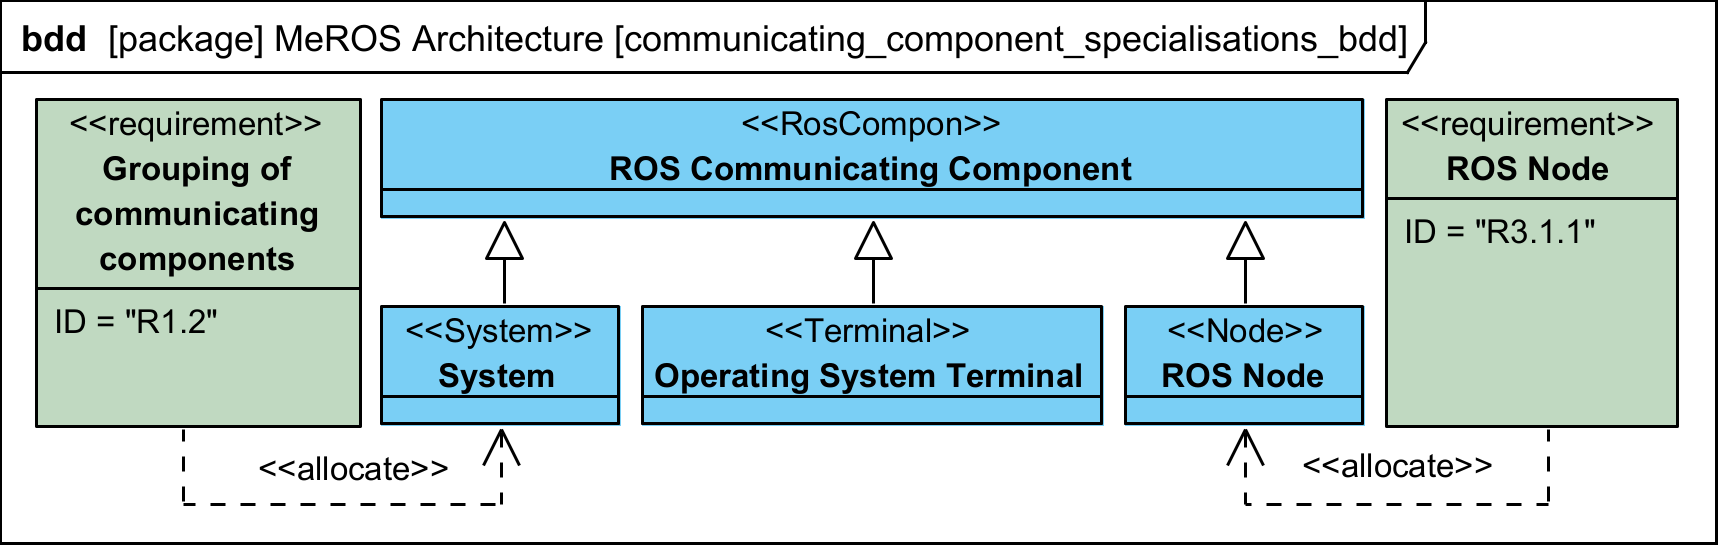
\includegraphics[scale=1.0]{diagrams/communicating_component_specialisations_bdd.png}}
		\end{center}
		\caption{Communicating Component and specialised blocks -- bdd.} 
		\label{fig:communicating_components_bdd}
	\end{figure}
	
	For clarity, relations of ROS Communicating Component are depicted in several diagrams. Fig.~\ref{fig:communicating_component_topics_bdd} considers Topics and their Data Structures. Here, the ROS Communicating Component can act as a~publisher or a~subscriber.	
	 
	
	\begin{figure}[H]
		\centering
		\begin{center}
			{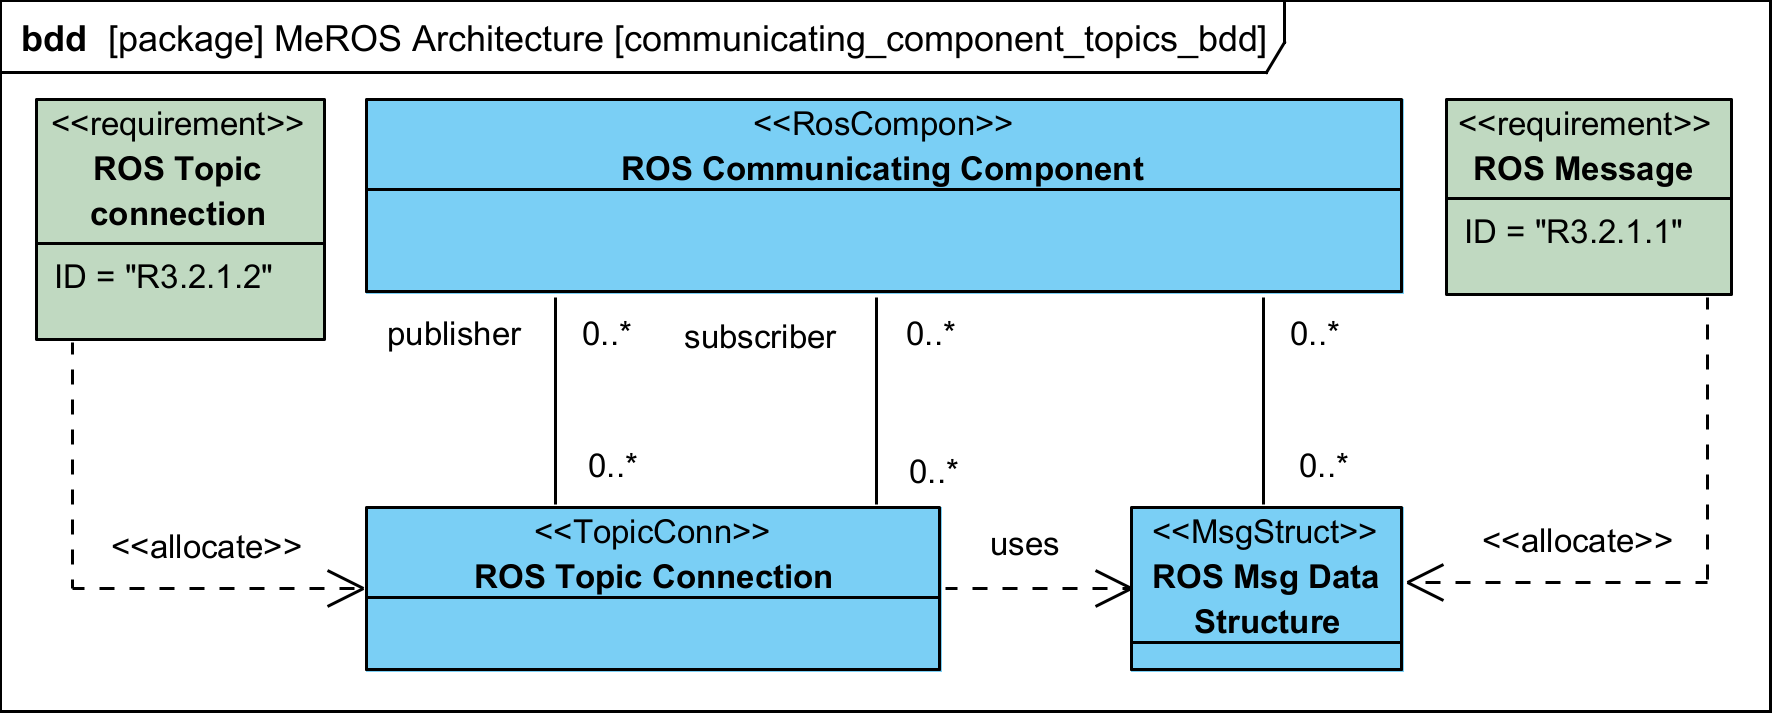
\includegraphics[scale=1.0]{diagrams/communicating_component_topics_bdd.png}}
		\end{center}
		\caption{ROS Communicating Component relations -- Topics.} 
		\label{fig:communicating_component_topics_bdd}
	\end{figure}
	
	\pagebreak
	
	Fig.~\ref{fig:communication_blocks_services_bdd} depicts Services and their Data Structures. In this case, the ROS Communicating Component can act as a~server or a~client.	
	
		
	\begin{figure}[H]
		\centering
		\begin{center}
			{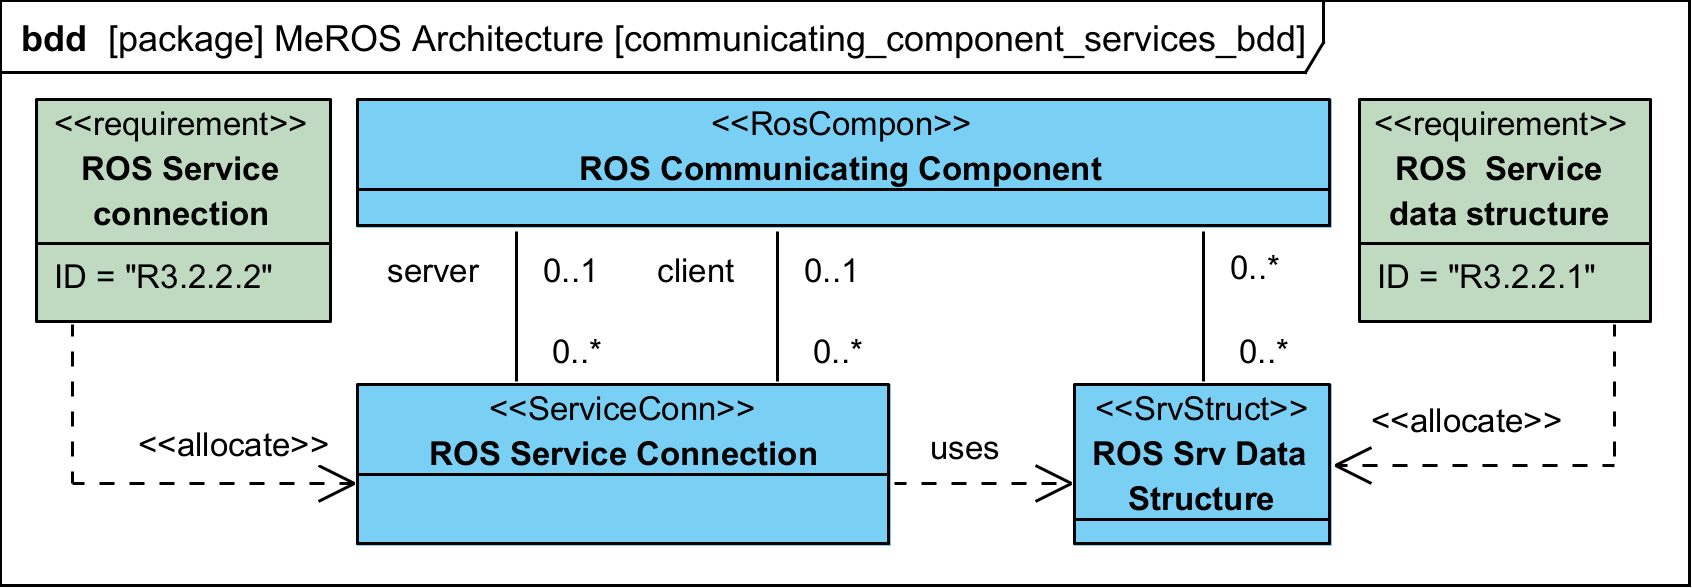
\includegraphics[scale=1.0]{diagrams/communicating_component_services_bdd.png}}
		\end{center}
		\caption{ROS Communicating Component relations -- Services.} 
		\label{fig:communication_blocks_services_bdd}
	\end{figure}
		
	The Actions are depicted in two diagrams -- Fig.~\ref{fig:communicating_component_actions_bdd} and Fig.~\ref{fig:action_bdd}. Similarly to Services, the ROS Communicating Component can act as a~server or a~client.	 
	
	
	\begin{figure}[H]
		\centering
		\begin{center}
			{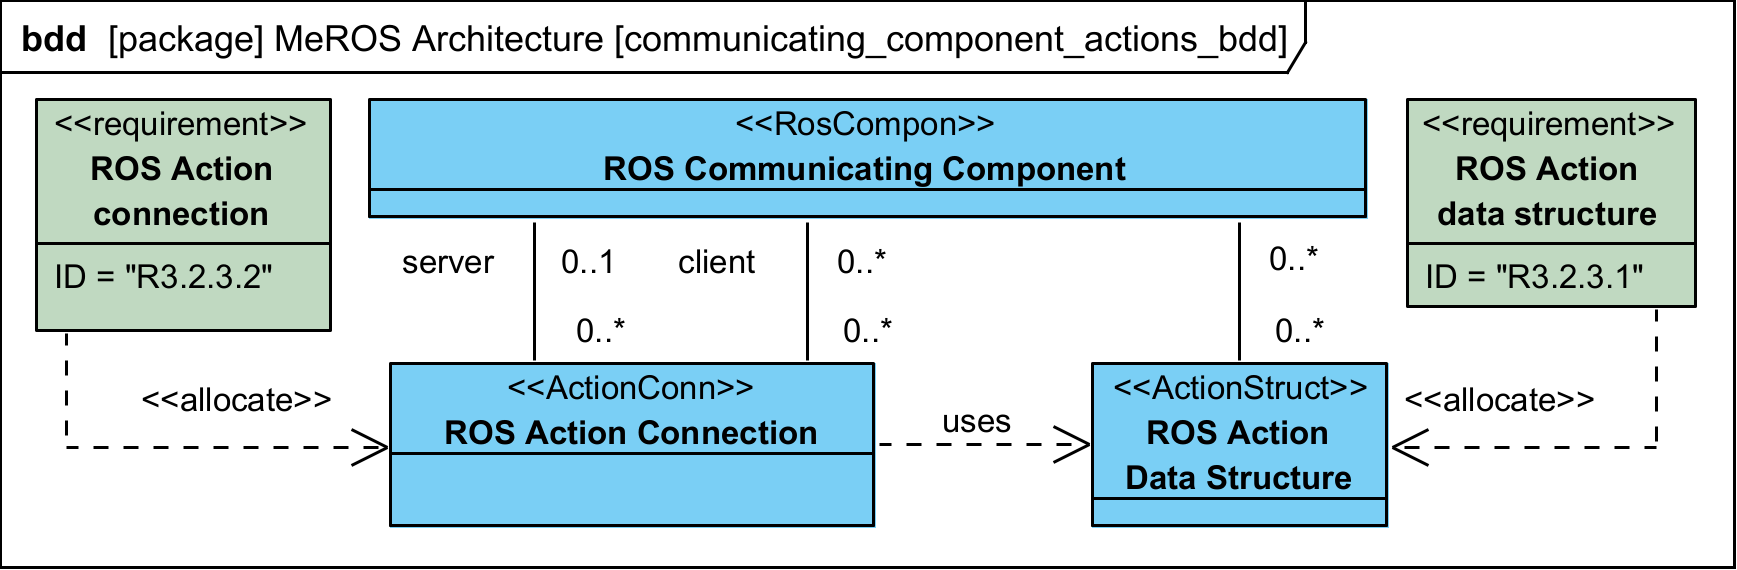
\includegraphics[scale=1.0]{diagrams/communicating_component_actions_bdd.png}}
		\end{center}
		\caption{ROS Communicating Component relations -- Actions.} 
		\label{fig:communicating_component_actions_bdd}
	\end{figure}
	
	The ROS Action Connection comprises two Topics and three Services (Fig.~\ref{fig:action_bdd}).
	
	\begin{figure}[hbt]
		\centering
		\begin{center}
			{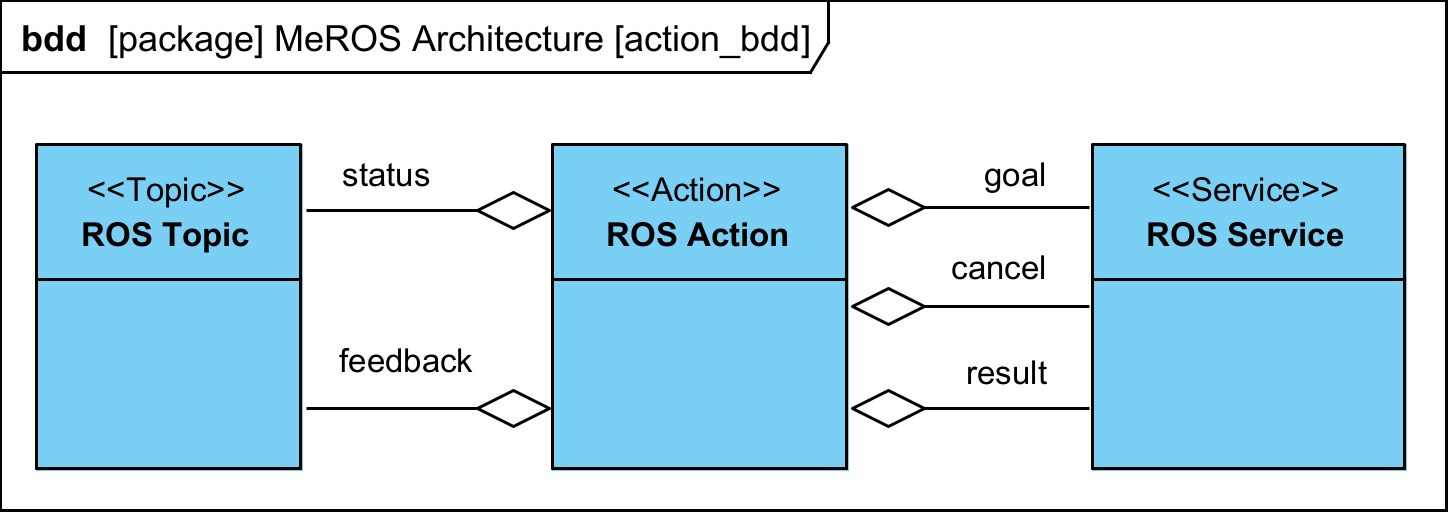
\includegraphics[scale=1.0]{diagrams/action_bdd.png}}
		\end{center}
		\caption{Action.} 
		\label{fig:action_bdd}
	\end{figure}
	
	\pagebreak
	
	The Communication Channel is introduced to specify communication between various Communicating Components (Fig.~\ref{fig:communication_channel_bdd}).
	Besides standard ROS communication methods, the Non-ROS can also be included (e.g., http request) to achieve interfaces with Non-ROS parts of the general system. 
	

	\begin{figure}[H]
		\centering
		\begin{center}
			{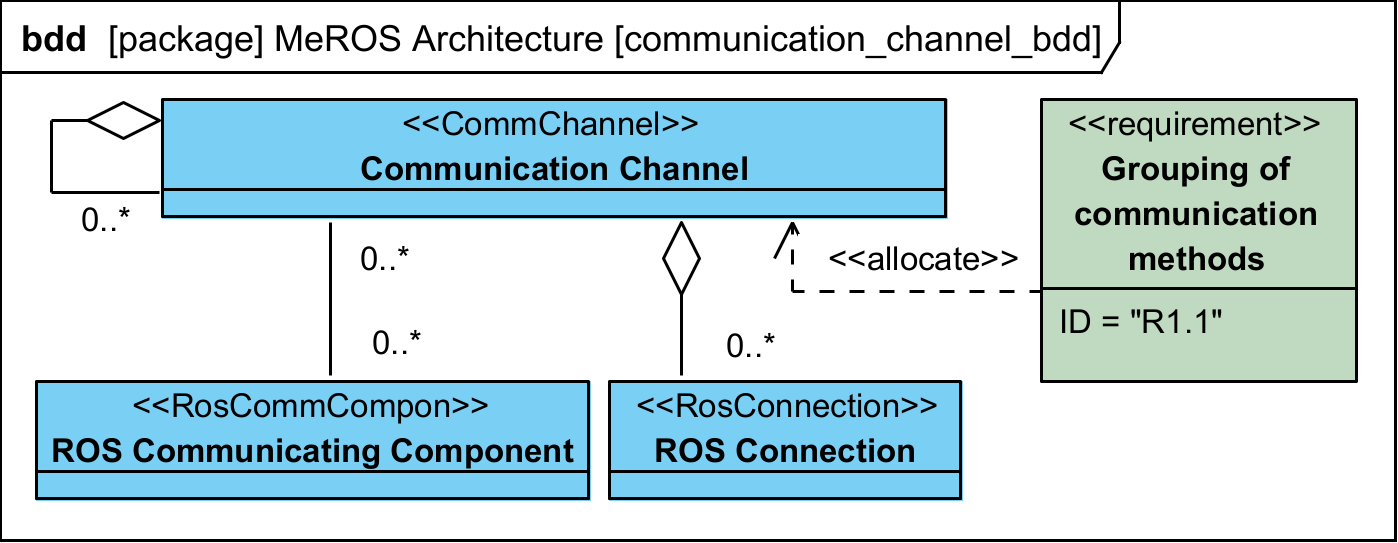
\includegraphics[scale=1.0]{diagrams/communication_channel_bdd.png}}
		\end{center}
		\caption{Communication Channel -- bdd.} 
		\label{fig:communication_channel_bdd}
	\end{figure}
	
		 
 	The Node (Fig.~\ref{fig:node_bdd}) composes Parameters. Component Container aggregates Nodes executed in a~single process. The Micro ROS Node is also considered in the model as the specialisation of the Node. 
 	
	 
 	\begin{figure}[H]
	 	\centering
	 	\begin{center}
	 		{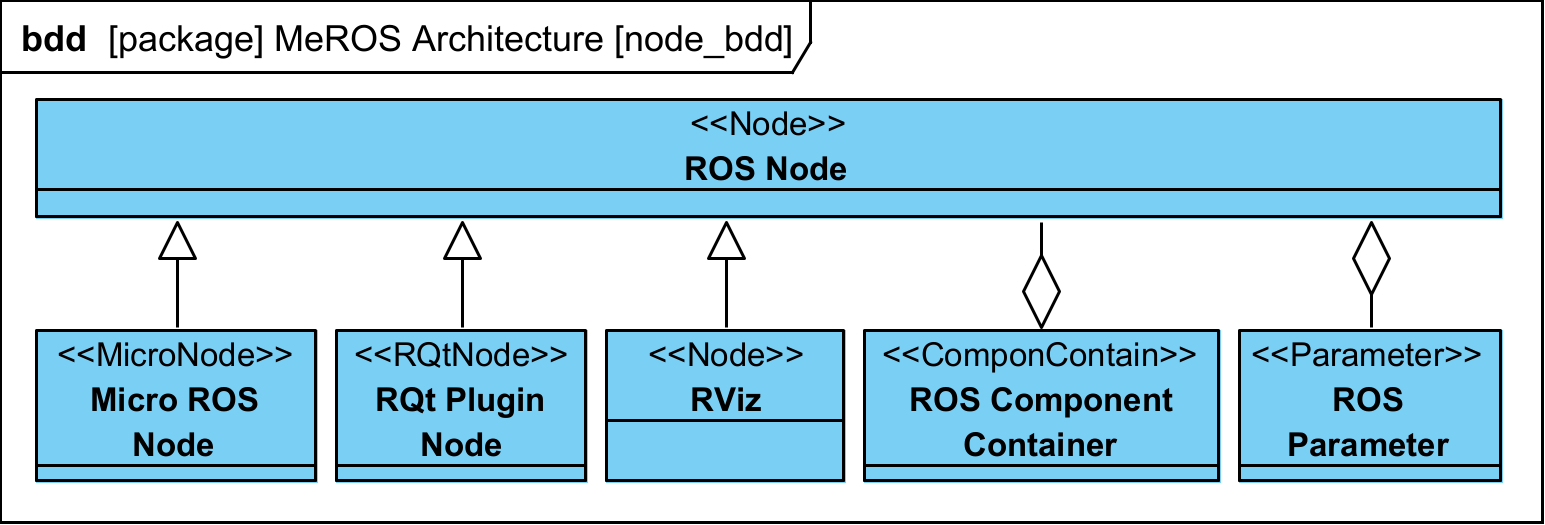
\includegraphics[scale=1.0]{diagrams/node_bdd.png}}
	 	\end{center}
	 	\caption{Node.} 
		 	\label{fig:node_bdd}
	 \end{figure}
	 
	The Running System Component (Fig.~\ref{fig:running_system_component_bdd}) is a~generalisation of Communicating Components specializations as well as Connections between them.
	

	\begin{figure}[H]
		\centering
		\begin{center}
			{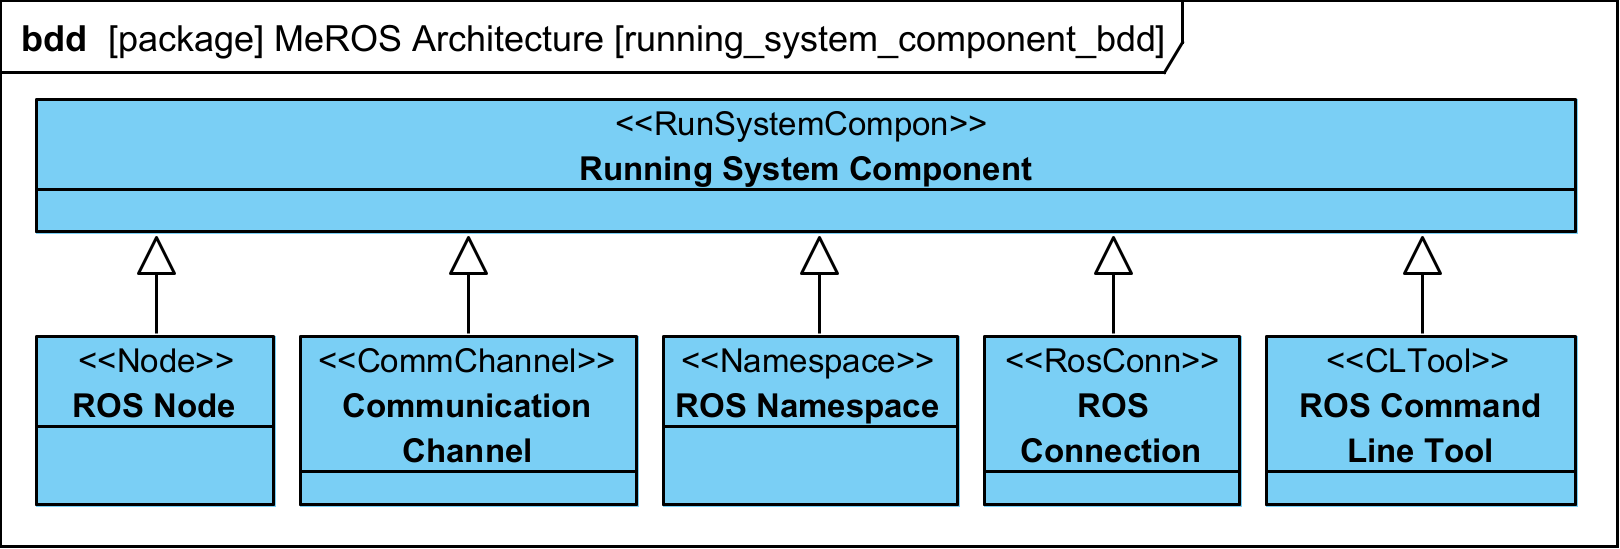
\includegraphics[scale=1.0]{diagrams/running_system_component_bdd.png}}
		\end{center}
		\caption{Running System Component specialisations.} 
		\label{fig:running_system_component_bdd}
	\end{figure} 
	 	 
	 \pagebreak	 
	 	 
	 The specializations of ROS connection (Topic connections, Service connections, and Action connections) are depicted in Fig.~\ref{fig:ros_connections_bdd}. 
	
	
	\begin{figure}[H]
		\centering
		\begin{center}
			{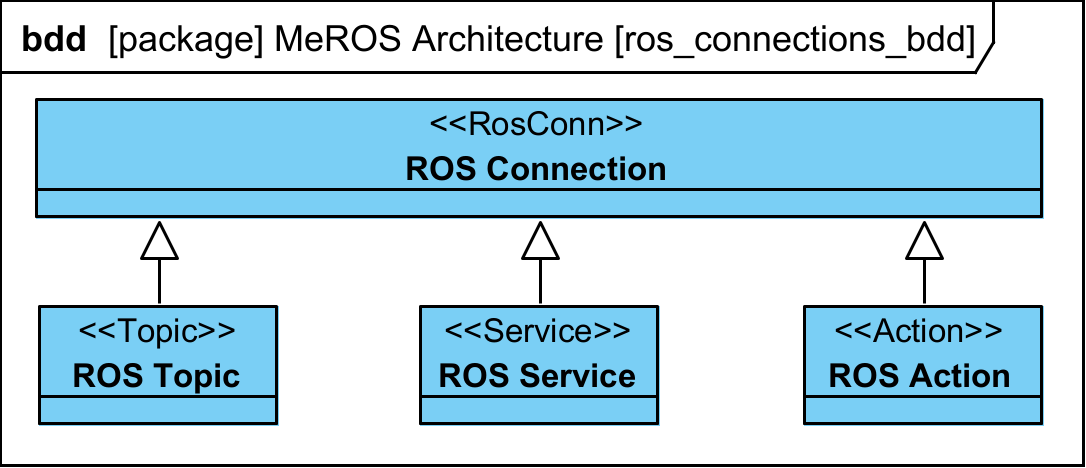
\includegraphics[scale=.94]{diagrams/ros_connections_bdd.png}}
		\end{center}
		\caption{ROS Connections.} 
		\label{fig:ros_connections_bdd}
	\end{figure}

	
	The Namespace (Fig.~\ref{fig:namespace_bdd}) aggregates elements of the System, but only ROS related. In opposition to the System, the Namespace does not specialise Communicating Component. Hence, it can not act as Communicating Component.
	
	
	\begin{figure}[H]
		\centering
		\begin{center}
			{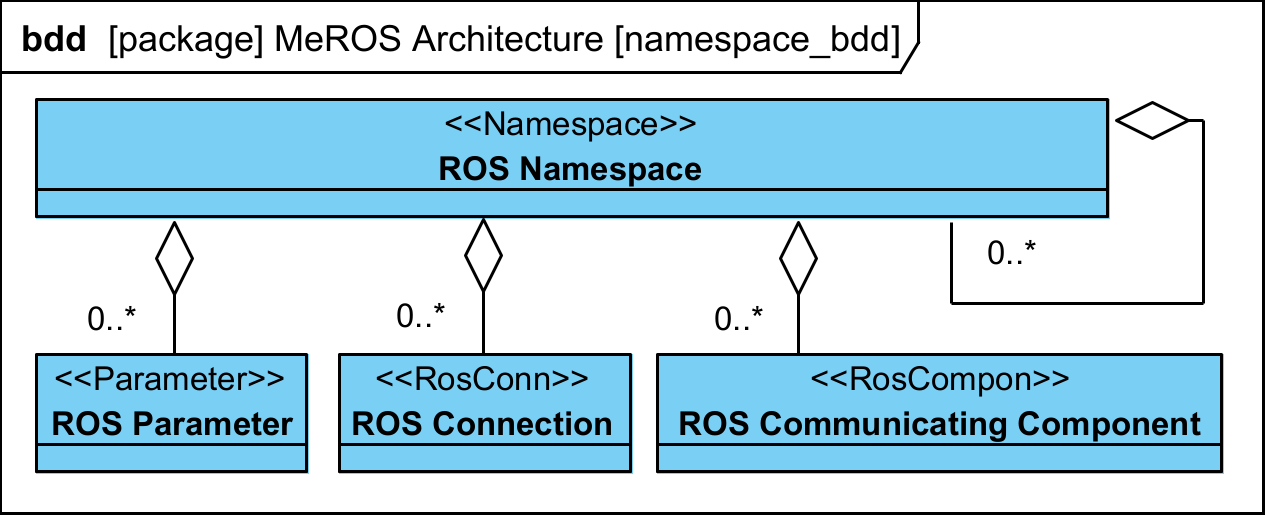
\includegraphics[scale=.94]{diagrams/namespace_bdd.png}}
		\end{center}
		\caption{Namespace composition.}
		\label{fig:namespace_bdd}
	\end{figure}
	
	The Sources Container (Fig.~\ref{fig:sources_container_bdd}) has various specialisations such as Group of Packages, ROS Workspace, ROS Package and Repository. It also plays a~role of general container.  
	The Workspace contains, i.a., Packages that compose the files related to general ROS concepts such as Node source codes, communication structures definitions, etc. As Workspace has a~specific file-system nature with various types of files stored, Group of Packages were introduced as specific aggregation of ROS Packages only.
	
	
	\begin{figure}[H]
		\centering
		\begin{center}
			{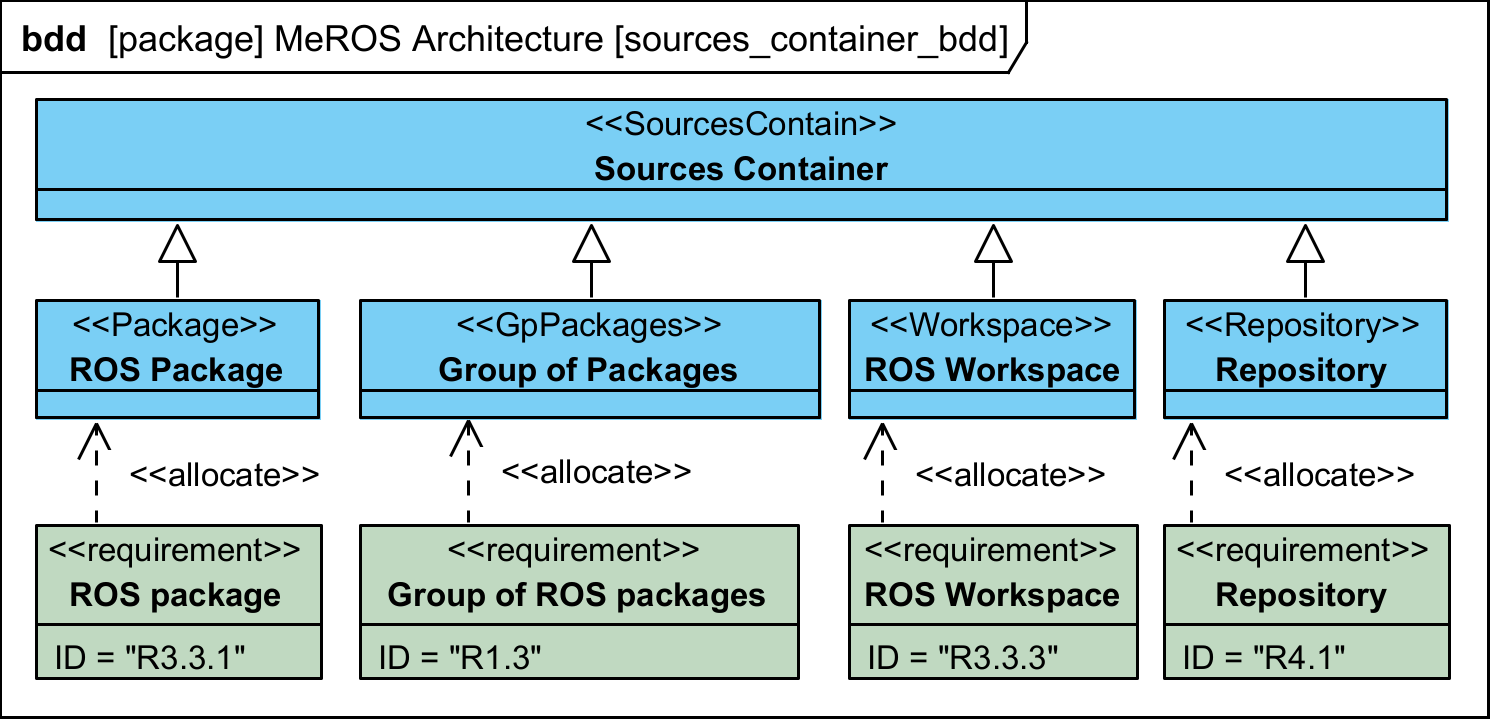
\includegraphics[scale=.94]{diagrams/sources_container_bdd.png}}
		\end{center}
		\caption{Sources Container and its specialisations.} 
		\label{fig:sources_container_bdd}
	\end{figure}
	
	The ROS Package (Fig.~\ref{fig:ros_package_bdd}) composes the files related to general ROS concepts such as Node source codes, communication structures definitions, etc. It should be noted that in case of Actions, specific communication structures definitions are stored in Action Data Structures. ROS Meta Package was introduced as a~specific ROS Package specialisation.
	
	\begin{figure}[H]
		\centering
		\begin{center}
			{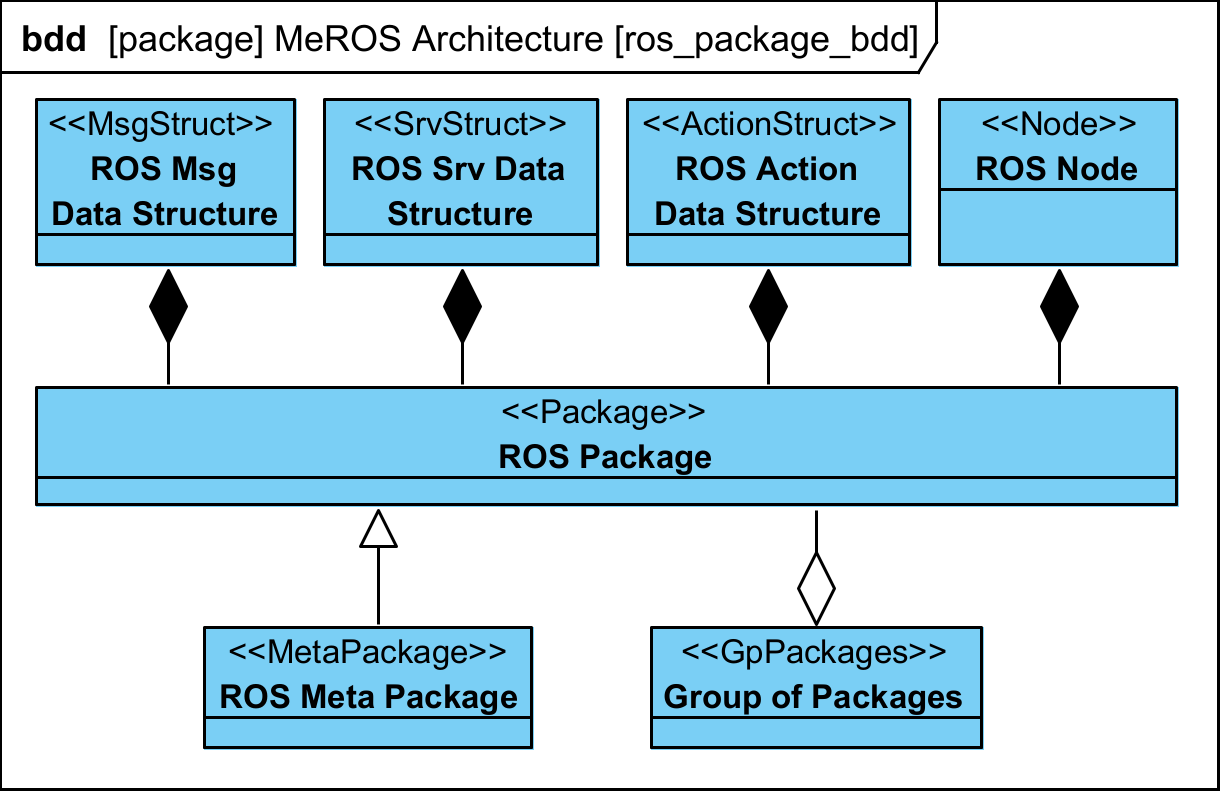
\includegraphics[scale=1.0]{diagrams/ros_package_bdd.png}}
		\end{center}
		\caption{ROS Package composition.} 
		\label{fig:ros_package_bdd}
	\end{figure}
		
The composition of Repository is presented in Fig.~\ref{fig:repository_bdd}.	
	
	\begin{figure}[H]
		\centering
		\begin{center}
			{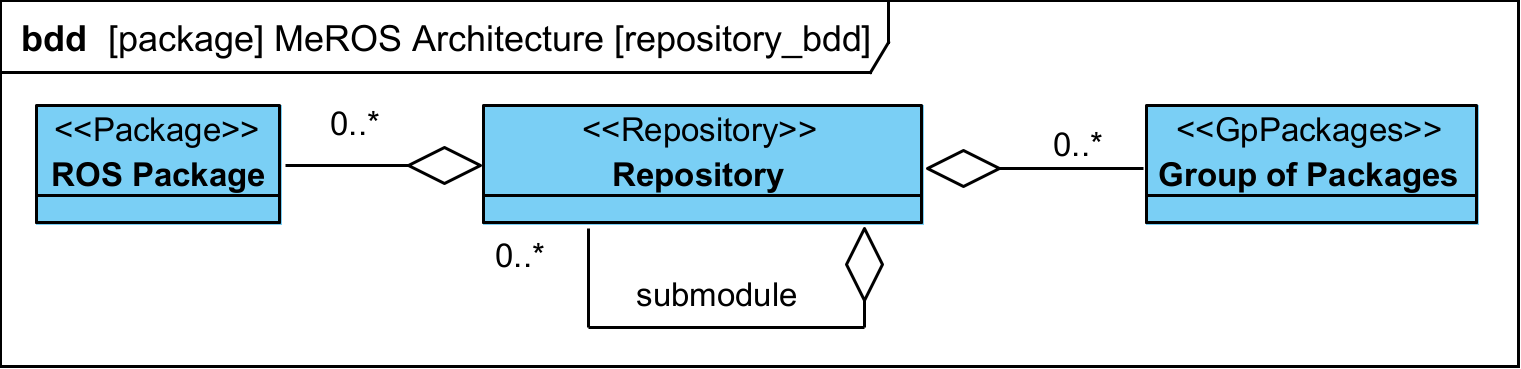
\includegraphics[scale=1.0]{diagrams/repository_bdd.png}}
		\end{center}
		\caption{Repository composition.} 
		\label{fig:repository_bdd}
	\end{figure}

The composition of ROS Workspace is presented in Fig.~\ref{fig:ros_workspace_bdd}.

	\begin{figure}[H]
		\centering
		\begin{center}
			{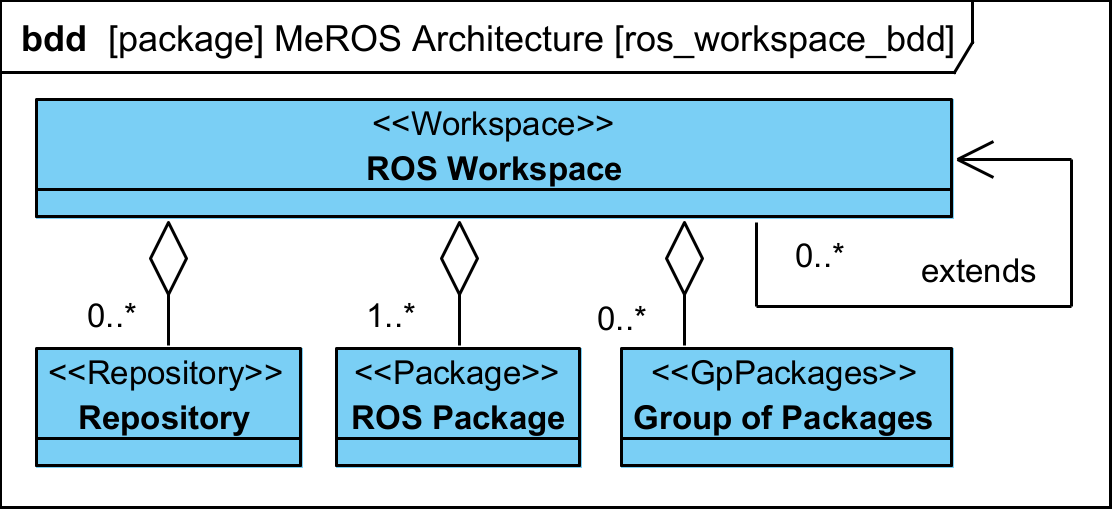
\includegraphics[scale=1.0]{diagrams/ros_workspace_bdd.png}}
		\end{center}
		\caption{ROS Workspace composition.} 
		\label{fig:ros_workspace_bdd}
	\end{figure}

			
\AtNextBibliography{\small}
\printbibliography
	
\end{document}
